\section{Event data format and the CMS software}
The particles produced during collision interact with various sub-detectors of 
the CMS experiment. The response of each sub-detector is stored in the form of
electronic signals. The physics objects from these electronic signals are
reconstructed following a chain of processes comprising many steps. The output 
data at every step are stored in a different format and serve as input for the 
subsequent steps. The detectors response is stored in the form of RAW data, which are further digitized (electronic response is converted into the energy 
deposits) and the output is stored in the form of DIGI data. The DIGI step itself 
involves various substeps such as RAW$\rightarrow$ DIGI$\rightarrow$ 
L1$\rightarrow$ DIGI2RAW$\rightarrow$ HLT $\rightarrow$ RAW2DIGI. The 
reconstruction algorithms are run on the DIGI data to reconstruct physics 
objects (see Chapter~\ref{c:secReco}). The data for the physics objects are 
stored in the form of RECO. The RECO data are further processed to get the 
analysis-specific objects and the output is stored in AOD (analysis object data) 
format. To reduce the size of AOD dataset as well as to retain only the most relevant 
physics objects, the AOD dataset is slimmed further and the output is stored in the 
form of a mini-AOD dataset. In this thesis, we have used the mini-AOD datasets. All 
the datasets are written on the disk with {\em .root} extension. The ROOT framework is 
used to browse the content of the root file.

The CMS software (CMSSW) is one of the most advanced packages which provides
thousands of sub-packages needed to analyze data at different steps. The CMSSW
is mostly written in C++ and python. The core design of the CMSSW relies on the 
event data model (EDM). All the sub-packages (modules) of the CMSSW run on each 
event separately, that is none of them run on two events at the same time. 
Different types of modules are available in the CMSSW to perform different types 
of operation. A schematic diagram of the event data model is shown in 
Figure~\ref{fig:cms_edm}. A brief description of these modules is given 
below.
\begin{itemize}[leftmargin=*]
\item \textbf{Source}: The source opens the root files and provides each event 
	to the subsequent modules. For the simulation where events are generated
	from scratch, an empty source is used. 
\item \textbf{EDProducer}: These modules take input from the input root file,
	perform some operations such as modifying physics objects, and put
	back the modified objects to the event. These modified objects are 
	further used by subsequent modules.
\item \textbf{EDFilter}: All the events of the input root file may not be needed
	for every analysis. In view of this, a set of filter modules are available
	in the CMSSW. These filters read the event and take the decision about 
	whether to keep that event or not. If the event is to be rejected then the 
	operation of the subsequent modules is halted. And the loop goes to the 
	next event. 
\item \textbf{EDAnalyzer}: The EDAnalyzers are the most frequently used modules for
	the physics analysis. The mini-AOD datasets contain all the relevant
	physics objects and the same dataset is used in every physics analysis. 
	However, different physics analysis has a different final state, therefore,
	the full content of mini-AOD dataset is not needed for every analysis.
	The EDAnalyzers are used to slim the miniAOD dataset and keep only the
	analysis-specific physics objects. The EDAnalyzer reads the event, 
	selects desired objects and relevant kinematic properties and writes out the
	necessary information into private data format known as \verb|ntuple|.
\item \textbf{OutputModule}: The output module stores the output event after
	all the other modules are executed.
\end{itemize}
\begin{figure}
  \begin{center}
  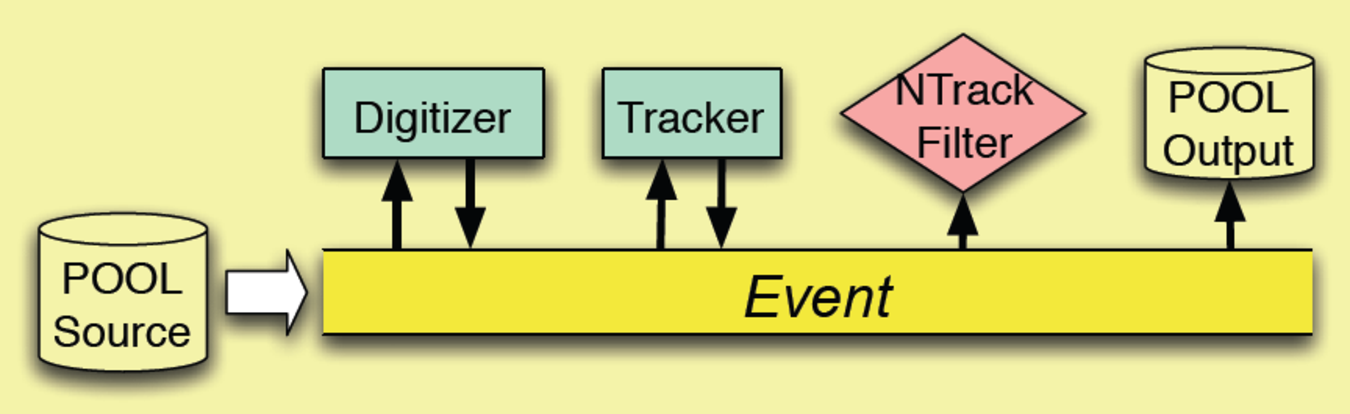
\includegraphics[width=0.75\linewidth]{Experiment/CMS/Image/cms_edm.pdf}
	  \caption{A schematic diagram of the event data model \cite{cmsEDM}. 
	  The {\em pool source} is a package that provides the input 
	  data for every event. The {\em digitizer} and {\em tracker } are the 
	  EDProducer which takes input from the event, do some operation and 
	  write the output to the same event. The {\em nTrack filter} is the
	  EDFilter which takes input from the event and decides if that event 
	  is to be kept or rejected. If the event is to be rejected then the
	  subsequent processing is halted and the CMSSW start looking at the next
	  event through {\em pool source}. The {\em pool output} package stores
	  the output after all the operations are performed.}
  \label{fig:cms_edm}
  \end{center}
\end{figure}

